\subsubsection{Статистика Ферми-Дирака.}
Т.к. электроны являются фермионами (частицами с полуцелым спином), то они подчиняются принципу исключения Паули, который утверждает, что в одном и том же состоянии может находится не более 1 фермиона, следовательно на одной орбитали может находиться не более 2-х электронов (с положительной и отрицательной проекцией спина).


Электроны, находясь в энергетическом уровне материалом (полупроводников в частности), находятся под влиянием электрического поля атома. Следовательно, система из достаточно большого количества электронов занимает (с учетом еще и теплового движения) такое состояние, которое обладает максимальной энтропией (или, если угодно, такое состояние, которое имеет наибольшую вероятность).


Таким образом, при нулевой температуре (а следовательно и нулевой тепловой энергии $kT = 0$) все электроны в полупроводнике находятся в валентной зоне, а зона проводимости пуста.

Распределение в общем виде, являющееся функцией вероятности нахождения электрона (фермиона) на уровне с энергией, равной $E$, является функция распределения Ферми-Дирака
\begin{equation}
F_n(E) = \frac{1}{e^{\frac{E-E_{\phi}}{kT}}+1}
\end{equation}
\begin{equation}
F_n(E) = \frac{1}{e^{\frac{\phi - \phi_F}{\phi_t}}+1}
\end{equation}
Где $\frac{kT}{q} = \phi_t$ -	 тепловой потенциал $ \phi_t(300 K)\approx 0.025 mV$\\

При этом, концентрация самих энергетических уровней в зонах вообще говоря неравномерна и подчиняется следующему закону распределения, выражающему плотность энергетических уровней на промежутке $d\phi$:
\begin{equation}
P(\phi) = \frac{2}{\sqrt{\pi}} (\frac{2 \pi q m^*}{h^2})^{3/2} \sqrt{\phi - \phi_{gr}}
\end{equation}
Где $\phi_{gr} = \frac{E_{gr}}{q}$, где $E_{gr}$ - граничная энергия (потенциальная энергия частицы на границы раздела зоны).\\ 
Где $\phi = \frac{E}{q}$, где $E$ - полная энергия, отсчитываемая от граничной.\\
Где $m^*$ - эффективная масса электрона, т.е. его масса в атоме (отличающася от массы электрона в вакууме )\\

\begin{center}
	\begin{figure}[H]
		\center{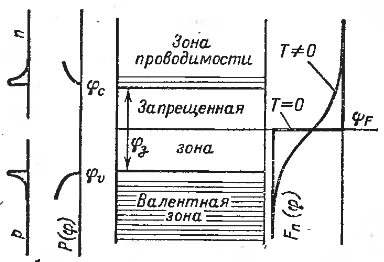
\includegraphics[scale=0.8]{fermi.png}}
		\caption{Распределение ферми, зоны, распределения уровней}	
  		\label{img:fermi}
	\end{figure}
\end{center}	


Полупроводники, для которых верно утверждение, что уровень Ферми находится внутри запрещенной зоны называются невырожденными. Для несобственных полупроводников справедливо, что $\phi - \phi_f > 0$, следовательно $F_n$ упрощается до $F_n = e^{-\frac{\phi - \phi_F}{\phi_t}}$. 


Концентрация электронов, находящихся в зоне проводимости определяется следующим интегралом:
\begin{equation}
n = 2 \int_{\phi_c}^{\infty} P(\phi - \phi_c) F_n(\phi) d\phi
\end{equation}
Где множитель 2 добавлен из-за того, что на одном уровне может находится 2 электрона с противоположными проекциями спина. А в распределении плотности уровней имеет место разность т.к. само значение $\phi$ в функции определяется относительно границы зоны\\

Решение этого интеграла имеет вид:
\begin{equation}
n = N_c  e^{-\frac{\phi_c - \phi_F}{\phi_t}}
\end{equation}
\begin{equation}
N_C = 2 (\frac{2 \pi m_n q  \phi_t }{h^2})^{3/2} \approx 0.5 * 10^{16} (\frac{m_n}{m}) T^{3/2} 
\end{equation}
\begin{equation}
np = N_c N_p e^{-\frac{\phi_z}{\phi_t}}
\end{equation}
Отметим, что произведение $np$ не зависит от уровня Ферми.\\
Для собственных полупроводников:
\begin{equation}
n_i = p_i = \sqrt{N_c N_p} e^{-\frac{\phi_z}{2 \phi_t}}
\end{equation}
Отсюда получаем, что 
\begin{equation}
np = n_i^2
\end{equation}

Плотность электронов в зоне проводимости определяет проводимость полупроводника.
Из данного уравнения следует, что концентрация носителей зарядов зависит от температуры ( она в основном определяет температурный потенциал в экспоненте) и ширины запрещенной зоны (которая определяется разностью $\phi_z = \phi_c - \phi_v$).  \\
Так например разница в ширине запрещенной зоны для германия и кремния (0.67 и 1.11 Вольт соответственно) приводит к разнице собственных концентраций (концентраций свободных носителей заряда (электронов в зоне проводимости)) на 3 порядка.

Уравнение $np = n_i^2$ дает возможность выразить концентрации n и p в разного рода полупроводниках (n и p типа) через собственную концентрацию.

\begin{equation}
n = n_i e^{-\frac{\phi_E - \phi_F}{\phi_t}}
\end{equation}
\begin{equation}
p = n_i e^{-\frac{\phi_F - \phi_E}{\phi_t}}
\end{equation}

Из этих же уравнений несложным логарифмированием можно выразить уровень Ферми, который лежит у проводников n-типа в верхней половине запрещенной зоны, для p-типа, соответственно, в нижней.\\



